Aplikacja webowa jest jedyną częścią systemu, do której użytkownik może mieć bezpośredni dostęp. Strona powstała w celu maksymalnego uproszczenia procesu badania kolejnych algorytmów i usług, które różniły się sposobem podawania danych wejściowych, sposobem uczenia oraz formatem zwracanych odpowiedzi. Do pozostałych zalet takiego rozwiązania należy ułatwienie przechowywania danych, poprzez umieszczenie ich we wspólnym miejscu co pomaga, w późniejszej interpretacji wyników.
\begin{figure}[H]
	\centering
	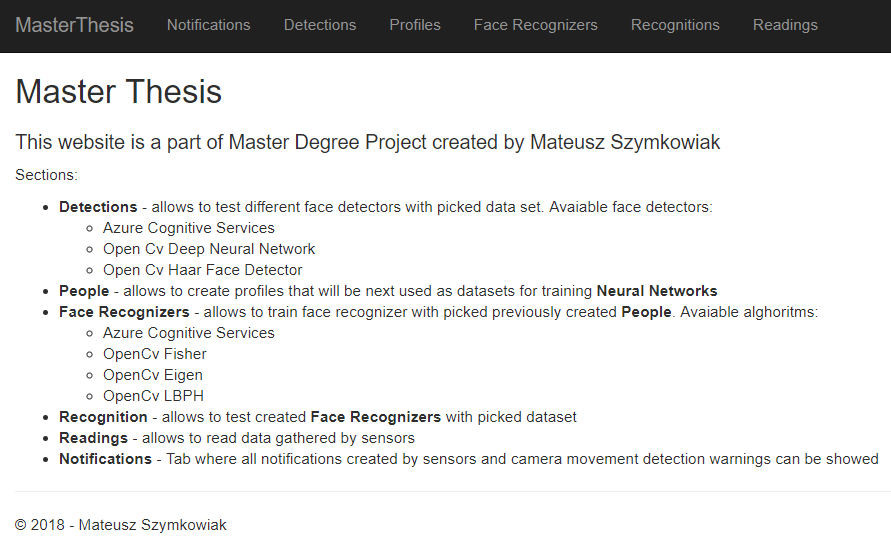
\includegraphics[scale=0.7]{aplikacja_webowa_razor_widok.png}
	\caption{Wygląd strony głównej aplikacji internetowej (rozwiązanie 1)}
	\label{fig:strona_glowna_razor}
\end{figure}
\pagebreak
Zgodnie z interfejsem przedstawionym na rysunku \ref{fig:strona_glowna_razor}, strona została podzielona na 5 głównych sekcji:
\begin{itemize}
\item Notifications- powiadomienia,
\item Detections- detekcje,
\item Profiles- profile tożsamości,
\item Face Recognizers- algorytmy rozpoznawania twarzy,
\item Recognitions- identyfikacja tożsamości,
\item Readings- odczyty sensorów.
\end{itemize}

\section{Technologie}\label{s:web_technologie}
Aplikacja webowa powstała w najnowszej kompilacji .NET Core 2, będącej międzyplatformową strukturą open source o wysokiej wydajności służącą do tworzenia nowoczesnych aplikacji internetowych opartych na usługach chmurowych. Logika biznesowa aplikacji została zaprogramowana w języku C\#. Warstwa widoku powstała w dwóch dostępnych rozwiązaniach, nieznacznie różniących się wyglądem, ale znacznie odbiegających od siebie sposobem działania. Przed omówieniem poszczególnych rozwiązań przedstawiono, krótkie definicje wykorzystanego wzorca projektowego MVC oraz technologii SPA. 

\subsection{Rozwiązanie 1- Razor Pages}
Pierwsza wersja została oparta o strony tworzone w technologi Razor Pages opartej o składnię Razor oraz podstawowe technologie webowe: HTML i CSS. Taki sposób tworzenia warstwy prezentacji jest zalecany dla aplikacji .NET Core, ponieważ pozwala zminimalizować ilość pracy wymaganej na jej utworzenie oraz zapewnia bardzo prosty proces wdrożenia. Aplikacja utworzona z pomocą Razor'a została zaprezentowana na rysunku \ref{fig:strona_glowna_razor}.

\subsection{Rozwiązanie 2- Angular 4}
Druga wersja widoku aplikacji oferuje dostęp do tych samych możliwości co pierwsze rozwiązanie, ale powstała przy pomocy frameworka webowego- Angular 4. Strona główna widoczna jest na rysunku \ref{fig:strona_glowna_angular}. Angular jest open sourcowym frameworkiem używanym do tworzenia aplikacji SPA (Single Page Application), napisany w języku TypeScript i wspierany oraz rozwijany przez Google.
\begin{figure}[H]
	\centering
	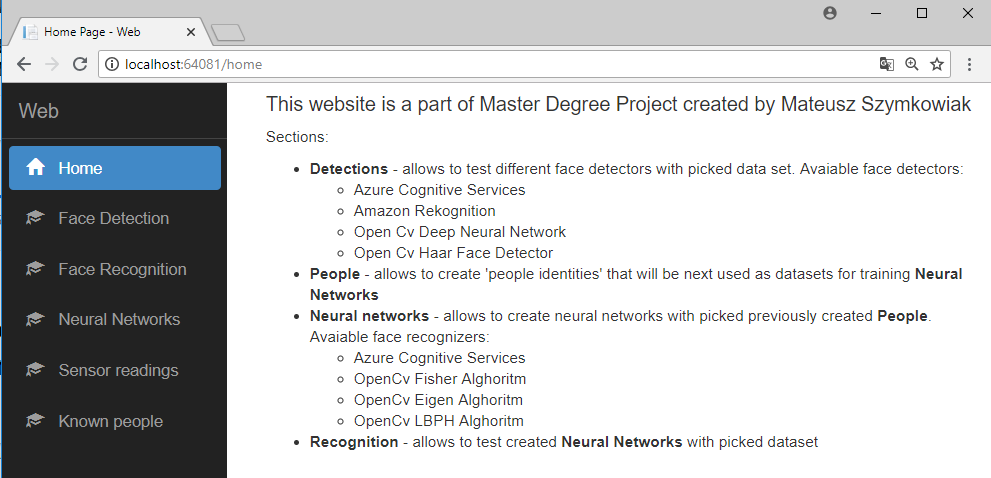
\includegraphics[scale=0.6]{aplikacja_webowa_angular_widok.png}
	\caption{Wygląd strony głównej aplikacji internetowej (rozwiązanie 2)}
	\label{fig:strona_glowna_angular}
\end{figure}

\section{Detekcja twarzy}
Detections jest stroną odpowiedzialną za wykrywanie twarzy na obrazach przesłanych do systemu. Na głównej stronie możemy zobaczyć wszystkie zlecone detekcje, zarówno nowe jak i już zakończone.
\begin{figure}[H]
	\centering
	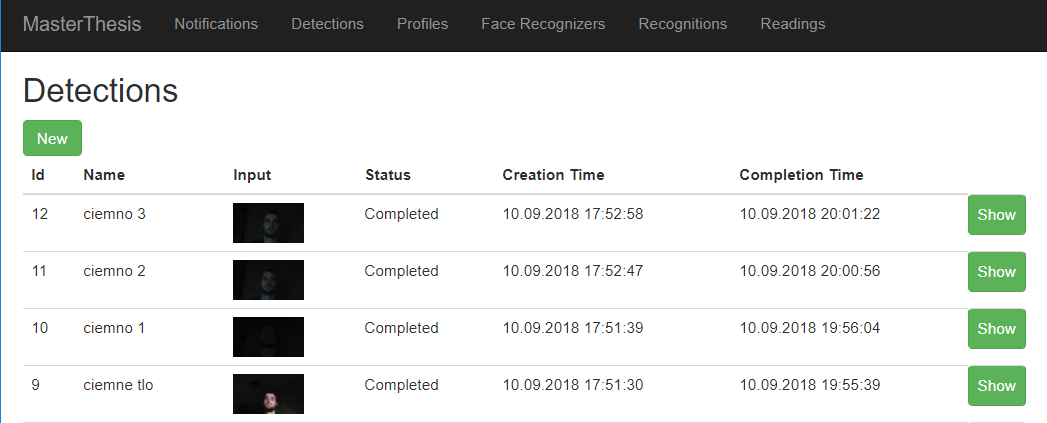
\includegraphics[scale=0.6]{detections.png}
	\caption{Widok detekcji twarzy}
	\label{fig:detections}
\end{figure}
Przycisk 'New' widoczny na \ref{fig:detections} pozwala na stworzenie nowego zadania wykrycia twarzy na obrazie, które zostanie przetworzone przez moduł aplikacji konsolowej. Na formularzu z rysunku \ref{fig:new_detection} należy podać nazwę zadania oraz za pomocą przycisku 'Wybierz plik' wybrać obraz w formacie png,jpg lub jpeg znajdujący się na dysku użytkownika.
\begin{figure}[H]
	\centering
	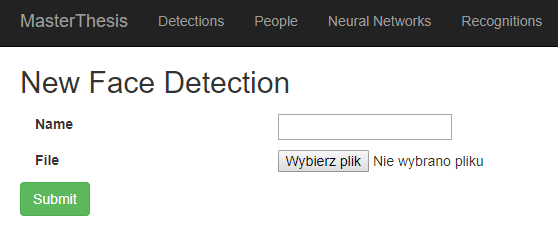
\includegraphics[scale=0.6]{new_detection.png}
	\caption{Tworzenie nowej detekcji}
	\label{fig:new_detection}
\end{figure}
Użycie przycisku 'Show' widocznego przy każdym zadaniu detekcji na rysunku \ref{fig:detections}, pozwoli na wyświetlenie szczegółów związanych z requestem, w tym wyników jeśli zadanie zostało zakończone.
\begin{figure}[H]
	\centering
	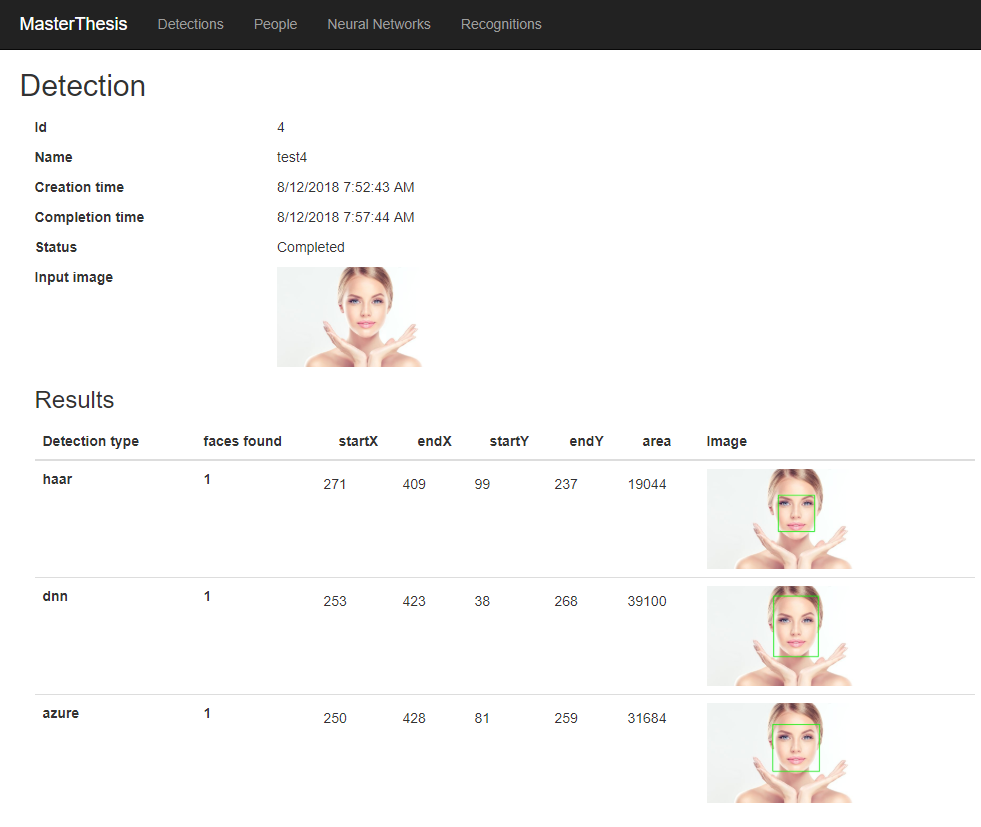
\includegraphics[scale=0.5]{detekcja_z_wynikami.png}
	\caption{Widok zakończonej detekcji}
	\label{fig:detekcja_zakonczona}
\end{figure}

\pagebreak

Strona ze zdjęcia \ref{fig:detekcja_zakonczona} pozwala sprawdzić datę utworzenia oraz zakończenia zadania, obraz wejściowy oraz tabelę z informacjami o wynikach detekcji, na które składają się:
\begin{itemize}
\item detection type- typ detekcji (haar, głęboka sieć neuronowa, azure),
\item faces found- ilość wykrytych twarzy,
\item processing time- czas potrzebny na wykrycie twarzy daną metodą,
\item startX, endX, startY, endY- współrzędne lewego dolnego oraz prawego górnego wierzchołka prostokąta obejmującego wykrytą twarz,
\item Area- rozmiar obszaru obejmującego twarz w pikselach.
\end{itemize}

\section{Profile}
Strona 'Profiles' służy do tworzenia nowych profili, które później mogą zostać wykorzystane jako dane uczące podczas trenowania wybranymi algorytmami. Do każdego profilu osoby musi zostać przypisany zasób minimum 2 zdjęć. W przypadku braku możliwości wykrycia twarzy na zdjęciu, zostanie ono zignorowane podczas procesu nauczania.
\begin{figure}[H]
	\centering
	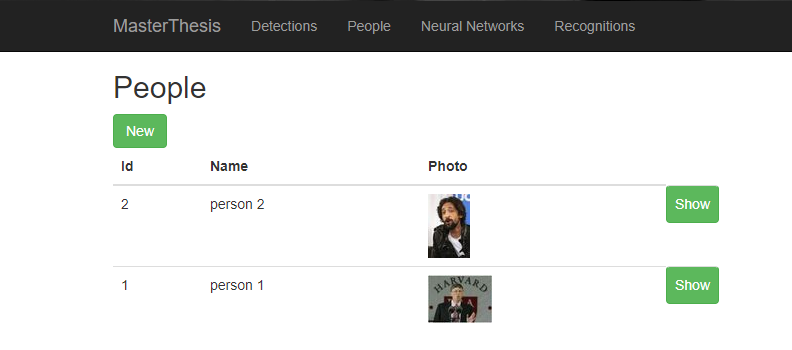
\includegraphics[scale=0.6]{people.png}
	\caption{Lista utworzonych profili}
	\label{fig:people}
\end{figure}
Nowa osoba może zostać utworzona w podobny sposób jak request detekcji twarzy. Jedyną różnicą jest wymóg wyboru kilku obrazów.
\begin{figure}[H]
	\centering
	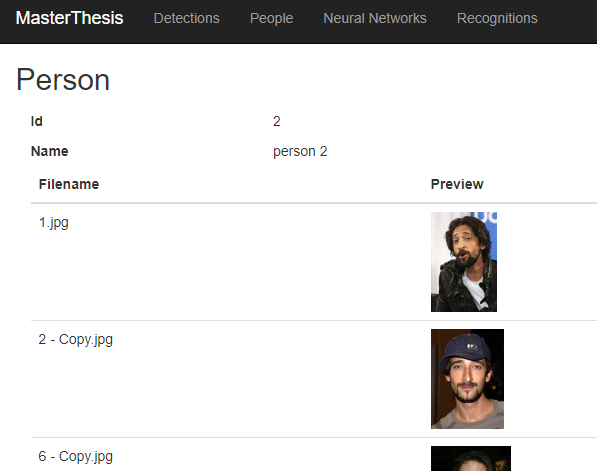
\includegraphics[scale=0.6]{person.png}
	\caption{Widok profilu}
	\label{fig:person}
\end{figure}
Utworzona osoba nie może być modyfikowana. Pierwsze załadowanie widoku osoby może trwać wydłużony czas z powodu procesu generowania linków do plików magazynowanych w usłudze Dropbox.

\section{Algorytmy rozpoznawania twarzy}
W zakładce 'Face Recognizers' użytkownik może utworzyć zadanie trenowania modelu wybranym algorytmem (OpenCv: Fisherfaces, Eigenfaces, LBPH, Azure: Cognitive Services) używając wybranej grupy profili z zakładki 'Profiles'. Użytkownik nie ma możliwości wyboru typu sieci, która zostanie nauczona. Domyślnie wszystkie dostępne rozwiązania (wymienione powyżej) zostaną wykorzystane.
\begin{figure}[H]
	\centering
	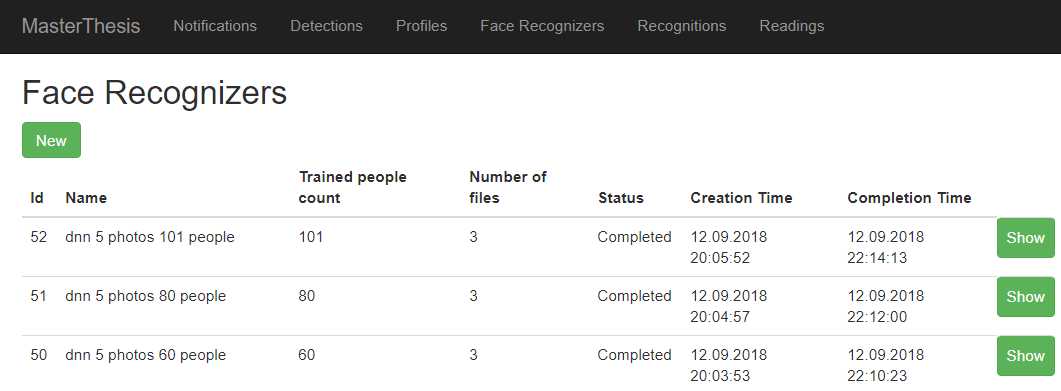
\includegraphics[scale=0.6]{neural_networks.png}
	\caption{Strona przedstawiająca istniejące grupy usług rozpoznawania tożsamości}
	\label{fig:sieci_neuronowe}
\end{figure}
Podczas tworzenia nowej sieci każdy istniejący profil zostanie wyświetlony jako checkbox, który należy zaznaczyć jeśli dany profil ma zostać wykorzystany w procesie nauczania. W wyniku szybkiego rozrostu bazy profili dodano checkbox 'Check all' pozwalający na wybranie wszystkich profili poprzez jedno kliknięcie. Kolejnym parametrem, który musi zostać wypełniony jest 'Photos per person used' określający maksymalną ilość zdjęć przypisanych do danego profilu, które mogą zostać wykorzystane do nauki sieci. Podana wartość powinna znajdować się w przedziale od 2 do 20. W przypadku gdy niedostępna będzie określana ilość zdjęć w danym profilu, to wykorzystane zostanie tyle zdjęć ile jest dostępnych.
\begin{figure}[H]
	\centering
	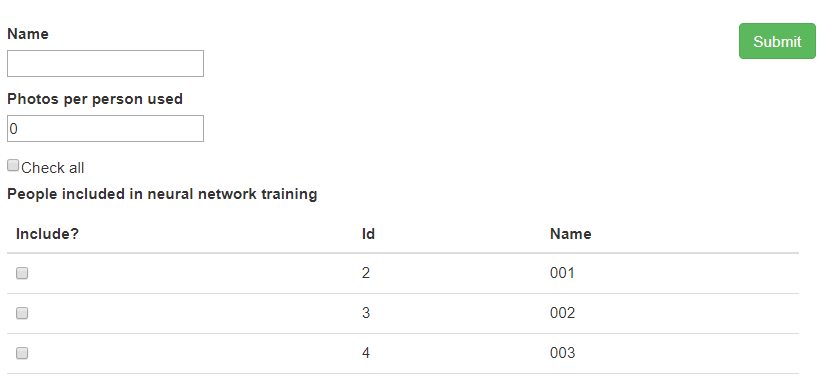
\includegraphics[scale=0.5]{nowa_siec.png}
	\caption{Tworzenie nowej grupy algorytmów identyfikacji twarzy}
	\label{fig:nowa_siec}
\end{figure}
Wykorzystując przycisk 'Show' z widoku na rysunku \ref{fig:sieci_neuronowe} można wyświetlić szczegółowe informacje o wybranej grupie sieci neuronowych. Dostępny widok ukazano na rysunku \ref{fig:siec_neuronowa}. Widoczne są na nim wszystkie parametry grupy,na które składają się: ilość wykorzystanych zdjęć i profili oraz tabela z informacjami o przygotowanych sieciach. Informacje dostępne w tabeli to nazwa i typ sieci, rozmiar utworzonego modelu, czas potrzebny na wytrenowanie oraz pełny czas(czas trenowania + przygotowanie danych wejściowych) potrzebny na stworzenie sieci.
\begin{figure}[H]
	\centering
	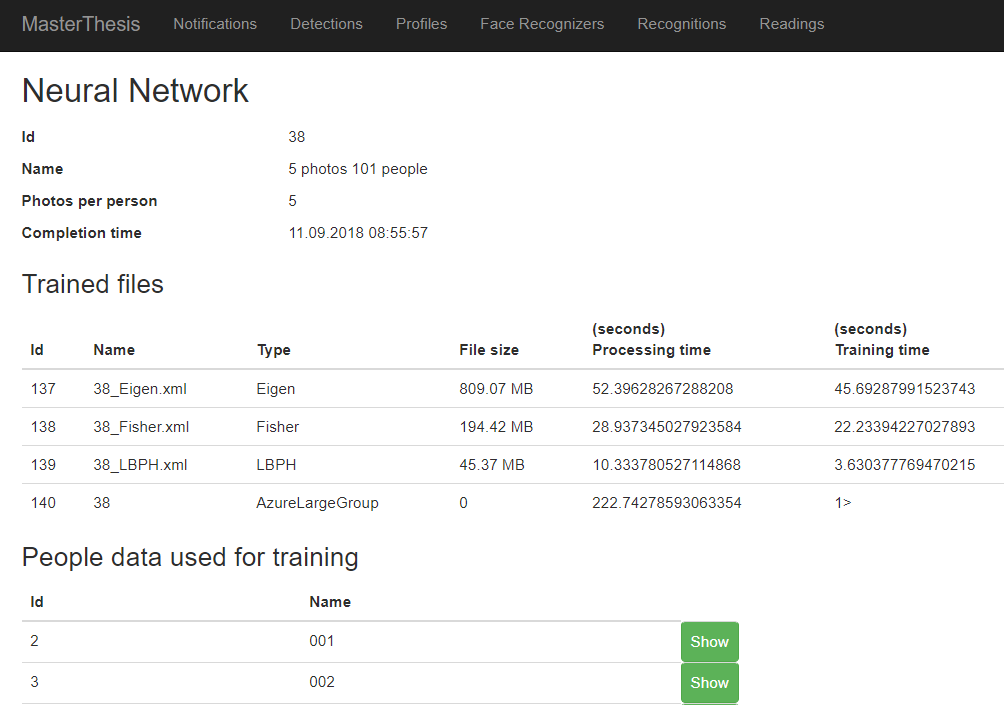
\includegraphics[scale=0.5]{siec_neuronowa.png}
	\caption{Szczegółowe informacje o utworzonej grupie}
	\label{fig:siec_neuronowa}
\end{figure}

\section{Rozpoznawanie tożsamości}
W sekcji 'Recognitions' użytkownik ma możliwość wykorzystać wcześniej utworzone zbiory identyfikatorów w celu rozpoznania tożsamości na zdjęciu przedstawiającym pojedynczą osobę.
\begin{figure}[H]
	\centering
	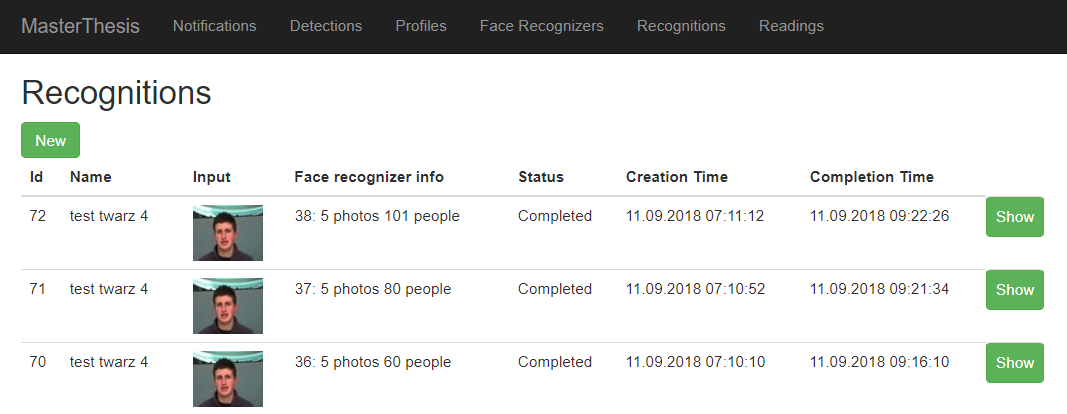
\includegraphics[scale=0.6]{recognitions.png}
	\caption{Lista zadań identyfikacji osoby}
	\label{fig:recognitions}
\end{figure}
Podobnie jak na pozostałych stronach, podczas tworzenia nowego zadania użytkownik będzie musiał uzupełnić prosty formularz. W formularzu przedstawionym na rysunku \ref{fig:new_recognition} należy załączyć jedno zdjęcie oraz wybrać grupę algorytmów trenowaną tymi samymi danymi, która ma zostać wykorzystana do identyfikacji tożsamości osoby.
\begin{figure}[H]
	\centering
	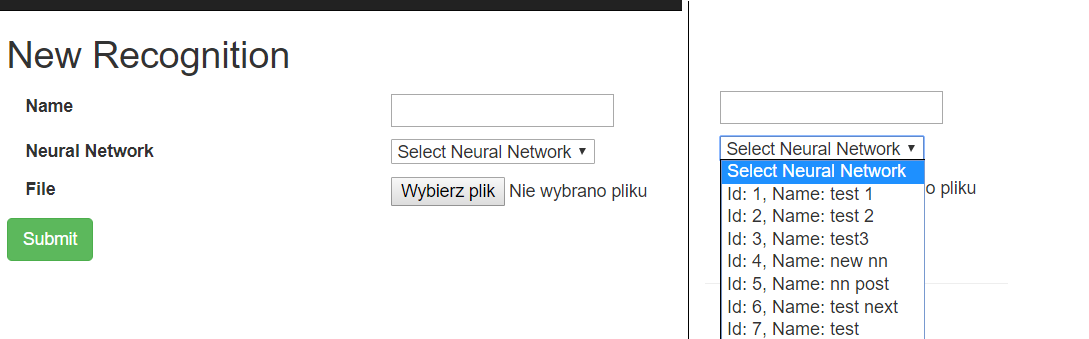
\includegraphics[scale=0.6]{new_recognition.png}
	\caption{Formularz tworzenia zadania identyfikacji}
	\label{fig:new_recognition}
\end{figure}
Po zakończonym procesie identyfikacji opisanym w kolejnym podrozdziale, użytkownik może wyświetlić wynik uzyskany przez każdą sieć dostępną w grupie. Przykładowy rezultat widoczny jest na zdjęciu \ref{fig:recognition}.
\begin{figure}[H]
	\centering
	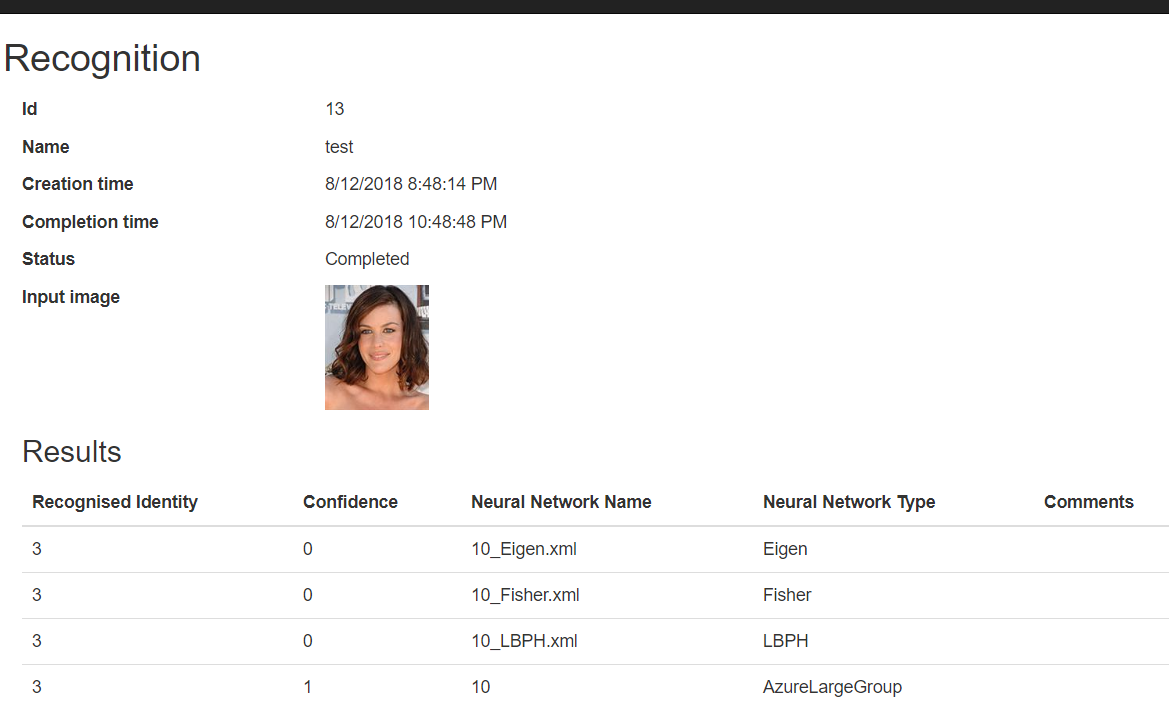
\includegraphics[scale=0.6]{recognition.png}
	\caption{Zakończony request identyfikacji}
	\label{fig:recognition}
\end{figure}

\section{Odczyty sensorów}
Zakładka Readings powstała w celu czytelnej prezentacji odczytów zebranych z sensorów w dniach funkcjonowania systemu. Odczyty zbierane są co minutę co generuje znaczną ilość wpisów do wyświetlenia. Z tego powodu po wejściu na stronę należy wybrać dzień, którym zainteresowany jest użytkownik. Przykładową listę zaprezentowano na rysunku \ref{fig:all_days}. Po wybraniu dnia ukazuje się widok, na którym przedstawiono wszystkie odczyty zebrane w wybranym okresie czasu.Do dostępnych informacji należą temperatura, wilgotność powietrza oraz czas wykonania pomiaru.
\begin{figure}[H]
	\centering
	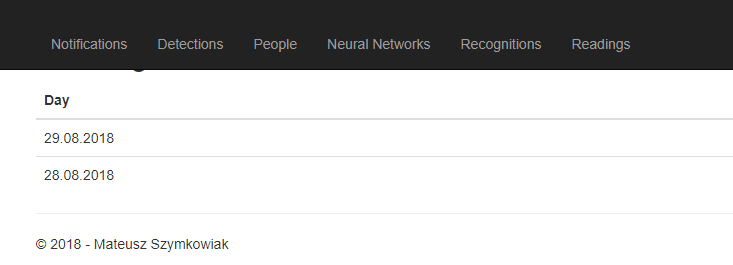
\includegraphics[scale=0.7]{all_days.png}
	\caption{Widok pozwalający na wybór dnia}
	\label{fig:all_days}
\end{figure}
\begin{figure}[H]
	\centering
	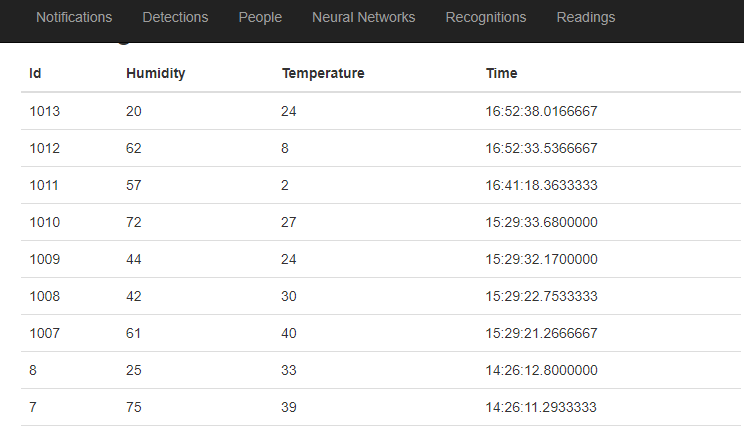
\includegraphics[scale=0.7]{daily_readings.png}
	\caption{Widok wyświetlający wszystkie odczyty z wybranego dnia}
	\label{fig:daily_readings}
\end{figure}

\section{Powiadomienia} \label{notifications}
Ostatnią ze stworzonych zakładek są Powiadomienia. Widok służy do wyświetlania wszystkich powiadomień utworzonych przez system, na które składają się powiadomienia sensorów oraz wykrycia ruchu.
\begin{figure}[H]
	\centering
	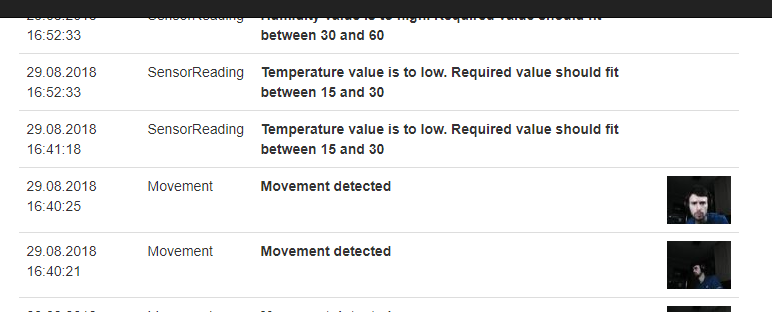
\includegraphics[scale=0.7]{notifications.png}
	\caption{Widok wyświetlający wszystkie odczyty z wybranego dnia}
	\label{fig:notifications}
\end{figure}
 Typy oraz sposób ich generowania zostały szerzej opisany w rozdziale \ref{aplikacja_zarzadzanie}. Każde wyświetlane powiadomienie posiada wiadomość,typ oraz czas utworzenia. W przypadku wykrycia ruchu dodatkowo wyświetlone zostaje zdjęcie uchwyconego wydarzenia. Kilka przykładowych powiadomień można zaobserwować na rysunku \ref{fig:notifications}.
 
